\begin{problema}{Hardwood Species}{Standard}{Standard}{UVa}


\noindent\begin{minipage}{.80\textwidth}
  { 
  Hardwoods are the botanical group of trees that have broad leaves, produce a fruit or nut, and generally go dormant in the winter.\\
  
  America's temperate climates produce forests with hundreds of hardwood species -- trees that share certain biological characteristics. Although oak, maple and cherry all are types of hardwood trees, for example, they are different species. Together, all the hardwood species represent 40 percent of the trees in the United States. \\
  }
\end{minipage}%
\begin{minipage}{.20\textwidth}
  \centering
  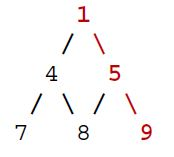
\includegraphics[height=3cm]{graficos/tree}
\end{minipage}
\\
\\
On the other hand, softwoods, or conifers, from the Latin word meaning ``cone-bearing'', have needles. Widely available US softwoods include cedar, fir, hemlock, pine, redwood, spruce and cypress. In a home, the softwoods are used primarily as structural lumber such as 2x4s and 2x6s, with some limited decorative applications. \\

Using satellite imaging technology, the Department of Natural Resources has compiled an inventory of every tree standing on a particular day. You are to compute the total fraction of the tree population represented by each species. \\

The first line is the number of test cases, followed by a blank line. Each test case of your program consists of a list of the species of every tree observed by the satellite; one tree per line. No species name exceeds 30 characters. There are no more than 10,000 species and no more than 1,000,000 trees. There is a blank line between each consecutive test case. \\

For each test case print the name of each species represented in the population, in alphabetical order, followed by the percentage of the population it represents, to 4 decimal places. Print a blank line between 2 consecutive data sets.\\

\Example

\input ejemplos/hardwood.txt

URL: \\ http://uva.onlinejudge.org/index.php?\\
option=onlinejudge\&page=show\_problem\&problem=1167

\end{problema}
